\subsection{Hard Disk}

La conservazione dei dati informatici all'interno dei vari elaboratori elettronici avviene con tecnologie e sistemi assai diversificati tra di loro. Questi dispositivi, che prendono il nome di ``Storage Devices'' sono spessi caratterizzati da numerose differenze sul piano fisico (Dischi magnetici, Nand, Flash, supporti ottici, nastri magnetici etc..) e sulla localizzazione (storage locali o remoti). 

Lo storage device considerato più comune rimane il supporto noto come Hard Disk (HD); si tratta di uno o più piatti metallici, ricoperti da un sottile film di materiale ferromagnetico. Le differenze elettromagnetiche rappresentano le informazioni coservate sotto forma di bit. 
L'organizzazione dei dati sui dischi è generalmente basata sul modello \textit{``Cylinder/Head/Sector''} o CHS (Cilindro/Testina/Settore).

\begin{itemize}
 \item Piatto
  \subitem Un HD è composto da più dischi paralleli; ogni superficie del disco corrisponde ad un piatto.
 \item Settore
  \subitem Un piatto è suddiviso in settori circolari; corrispondo a spicchi radiali sul piatto.
 \item Traccia
  \subitem Un piatto è suddiviso in porzioni ad anello concentriche
 \item Testina
  \subitem Su ogni piatto lavora una testina di lettura/scrittura; tutte le testine sono solidali tra loro.
 \item Cilindro
  \subitem Indica lo spazio descritto da tracce equidistanti dal centro su tutti i piatti del HD.
\end{itemize}

Ad ogni modo, nonostante gli hard disk siano strutturalmente complessi, il sistema operativo offre un notevole livello di astrazione che consente di poter sfruttare lo spazio di immagazzinamento come una area contigua ed organizzata secondo schemi di partizionamento. Lo schema di partizionamento preso in esame è quello noto come \textbf{``MSDOS''}.

\begin{figure}[!ht]
 \centering
 \includegraphics[scale=0.4]{Immagini/disk_scheme.png}
 \label{fig:DiskScheme}
 \caption{Schema Partizionamento}
\end{figure}

\subsubsection{M.aster B.oot R.ecord}

Il Master Boot Record (MBR) è quel settore del disco che contiene i primi 512 Byte del disco, noto anche come settore di avvio.  Al suo interno è suddiviso in 

\begin{itemize}
 \item 446 Byte: MBP Master Boot Program (stage1, lba48 pointer)
 \item 64 Byte: MBT Master Boot Table
 \item 2 Byte: Magic Number (AA 55)
\end{itemize}


Per quanto questo schema sia ampliamente utilizzato, mantiene anlcuni limiti legati ad un design datato rispetto all'evoluzione tecnica dei dispositivi di storage. 
Uno dei limiti fondamentali è legato al numero di partizioni primarie (4 al massimo); questa limitazione è in parte superata con l'adozione di partizione estese alle interno delle quali sono definibili 11 partizioni logiche. 


\subsubsection{Partizioni}

Lo spazio disponibile sul disco è suddivisibile in partizioni. Le partizioni, se pur caratterizzate per tipologie, rappresentano esclusivamente dei contenitori all'interno dei quali vengono creati dei filesystem. 
In questa fase è opportuno aver ben presente la differenza tra partizione, che è una suddivisione del dispositivo di storage, e filesystem che invece è una struttura dati atta ad organizzare i file all'interno del disco.

Nei sistemi Linux vengono utilizzati 3 tipi distinti di partizioni 

\begin{itemize}
 \item Linux (0x83): Utilizzata per i filesystem ext2/ext3/ext4 
 \item Linux swap 0x82: Utilizzata per le partizioni di swap
 \item Linux LVM 0x8e: Utilizzata per creare dei Physical Volume LVM
\end{itemize}

Una delle regole ``non scritte'' del mondo GNU/Linux è che \textit{``everything is a file''} (tutto è un file), nel senso che tutto (o quasi) all'interno del sistema, attraverso opportuni strumenti di astrazione hardware, è visibile sotto forma di file. 
Non fanno eccezioni i vari dispostivi di storage (sd), che sono solitamente allocati all'interno della cartella \textbf{/dev}; ad esempio quello che sara visto come primo disco, sara indicato con \textbf{sda} il secondo \textbf{sdb} il terzo \textbf{sdc} e cosi via.
Meccanismo analogo vale per le partizioni all'interno del disco; la prima partizione prenderà il nome di \textbf{sda1}, la seconda \textbf{sda2} e così a seguire. 
Questo meccanismo, non univoco benchè assai intuitivo, offre un primo modo di identificare dischi e partizioni per eseguire le operazioni basilari.

\subsubsection{Filesystem}

Il filesystem è la struttura dati con cui sono organizzati i dati all'interno del dispositivo di storage. Tale organizzazione varia molto sulla base del sistema operativo utilizzato; ad esempio le versioni passate dei sistemi operativi Microsoft\textregistered utilizzano una struttura nota come \textit{``Tabella di allocazione File''} (\textbf{FAT}: File Allocation Table), mentre i sistemi Unix e derivati si basano su una sistema basato su \textbf{inode}. 

I filesystem trattati in questo testo sono:

\begin{itemize}
 \item ext2: Second Extended Filesystem
 \subitem: Filesystem basato su inode, semplice e prestazionale sulle piccole dimensioni 
 \item ext4: Fourth Extended Filesystem
 \subitem Evoluzione di ext3, 48bit, journaled, default dei sistemi GNU/Linux odierni.
 \item FAT: File Allocation Table
 \subitem Filesystem molto semplice di derivazione Microsoft\textregistered, limitato
 \item xfs: XFS, Silicon Graphics
 \subitem Filesystem 64bit, B-tree+, ideale per grandi volumi
 \item glusterfs
 \subitem Filesystem ideato per lavorare su sistemi cluster
\end{itemize}

A seguire alcune caratteristiche notevoli dei filesystem presi in considerazione

\begin{center}
\begin{tabular}{|l|ccr|}
\hline
 & Max. File & Max. Vol.  & FilenameChar \\
\hline
ext2 (1K) & 16 GiB & 2 TiB & 255 \\
ext2 (8K) & 2 TiB & 32 TiB & 255 \\
ext4 & 16 TiB & 1 EiB & 255 \\
xfs & 8 EiB & 16 EiB & *\\
FAT32 & 4GiB & 124/2048 GiB & 255 \\
\hline
\end{tabular}
\end{center}



\subsubsection{Mount Point}

A differenza dei sistemi operativi Microsoft\textregistered, dove di solito le partizioni vengono indicate con il nome di unita logiche (es. C:, D: etc..), per utilizzare i vari filesystem (locali e remoti) è necessario ``montarli'' su un percorso all'interno dell'abero delle cartelle. 
Al momento dell'avvio del sistema viene impostata la cartella radice (root directory indicata con \textbf{``/''}, da non confondere con la cartella dell'utente root che si trova su \textbf{``/root''}.
Tutti i filesystem montati successivamente saranno visibili in sotto directory della cartella radice specificate al momento del mount. Alcune cartelle sono di solito dedicate a questa funzione come la \textbf{/mnt} o per i media removibili su \textbf{/media}. Ciò vale anche per supporti esterni quali CD/DVD, USB Mass Storage e filesystem di rete (es. NFS e CIFS).


\subsubsection{Disk Utility}

\begin{figure}[!ht]
 \centering
 \includegraphics[scale=0.4]{Immagini/Disk_Utility1.png}
 \label{fig:DiskUtility}
 \caption{Disk Utility}
\end{figure}

Per la gestione delle partizioni, all'interno del sistema è presente la \textbf{``Disk Utility''}, uno strumento dalla grafica intuitiva, che consente di identificate il disco interessato, creare, rimuovere modificare partizioni, formattarle e stabilire un punto di mount. 

\subsubsection{Comandi per partizioni e filesystem}

TODO

\subsection{LVM}

\begin{figure}[!ht]
  \centering
  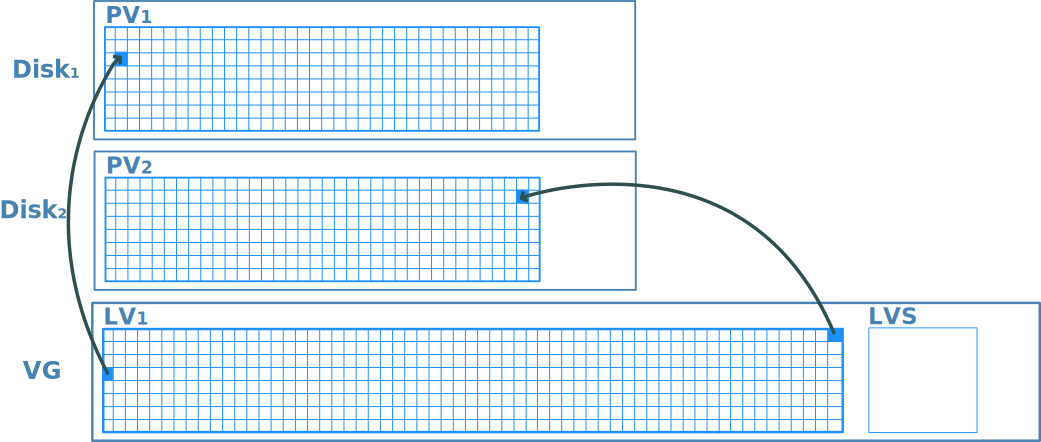
\includegraphics[scale=0.4]{Immagini/partitions.png}
  \label{fig:LVM_scheme}
  \caption{Volume Group composto da due Physcal Volume}
\end{figure}



Il Logical Volume Manager è uno stato software che crea un livello di astrazione più alto sopra dischi e partizioni, tale da superare i limiti imposti dal livello fisico, offrendo continuità tra dischi differenti, flessibilità ed affidabilità.

All'interno del LVM è utile identificare gli elementi che lo compongono

\begin{itemize}
 \item PP: Physical Partition
 \subitem Partizione fisica di tipo Linux LVM (0x83).
 \item PV: Physical Volume
 \subitem I physcal volume sono le PP inizializzate che andranno a comporre il volume group.
 \item VG: Volume Group
 \subitem L'astrazione a livello software che mostra tutti i physical volume con un unico dispositivo di storage. Lo spazio al suo interno è diviso in \textbf{``extens''}, che devono essere di dimensione omogenea tra i vari PV. 
 \item LV: Logical Volume
 \subitem Rappresentano le ``partizioni'' all'interno del Volume Group. Sono estensibili e formattabili con i filesystem ext4. 
 \item PE: Physical Extens
 \subitem Sono i blocchi funzionali con cui i VG mappano lo spazio di allocazione sui vari PV. Le dimesione dei PE è variabile in base al tipo di prestazioni che si vogliono enfatizzare.  
 \item LE: Logical Extens
 \subitem Sono i blocchi funzionali di mappatura ta il LV ed il VG. A meno che i PV non siano configurati in ``mirror'', ad ogni LE, corrisponde un PE. 
\end{itemize}

L'utilizzo di LVM consente facilmente di superare i limiti legati agli schemi di partizionamenti tradizionali in termini di numero di partizioni, ma anche di dimensione allocabile (il VG, nella configurazione normale, è uguale alla somma dei PV che lo compongono, a meno di configurazione ``mirror''). 
Inoltre, il superiore livello di astrazione consente all'amministratore di variare la dimensione del LV, modificando il filesystem in esso contenuto. 
Tale operazione, nel caso si tratti di una \textbf{estensione} è generalmente considerata sicura, ed è effettuabile anche a caldo (ovvero quando il filesystem che insiste su LV risulta montato). Ciò non è altrettanto vero parlando di \textbf{riduzione}, dove per varie ragioni tecniche, è raccomandabile eseguire un backup dei dati contenuti, e non è possibile effetturare questa operazione a caldo. 
Un'altra potrnzialità ovverta da LVM, è la possibilità di creare degli Snapshot (LVS); uno snapshot è una sorta di immagine virtuale di un LV in utilizzo, realizzato dedicando una area del volume group apposita, dove vengono salvate solo le versioni originali dei file modificati.
Qualora le modifiche al LV risulteranno valide è possibile scartare lo snapshot, in caso contrario è possibile eseguire una operazione di merge che riporta alla configurazione ``fotografata'' al momento della creazione dello snapshot.

\subsubsection{Logical Volume Management}
%\textbf{System} $\rightarrow$ \textbf{Administration} $\rightarrow$ \textbf{LVM}

Questa applicazione, visibile nel menu sotto \menu{System > Administration > LVM} (nome applicazione: \textit{system-config-lvm}) consente di creare, gestire e modificare i Physical Volume, i Volume Group ed i Logical Volume.

\begin{figure}[!ht]
 \centering
 \includegraphics[scale=0.4]{Immagini/LVM_utility.png}
 \label{fig:LVM Utility}
 \caption{LVM Utility}
\end{figure}


\subsubsection{Comandi da terminale per LVM}

TODO

